
\section{Vectors}

\begin{definition}[]{Basics}
    Vector can be represented by $\vec{F}$ or $\boldsymbol{F}$. The magnitude can be represented by $|F|$ or $F$.
\end{definition}

\begin{knBox}[]{Unit vectors}
    They are vectors with magnitude 1. $\hat{A}=\frac{\vec{A}}{|\vec{A}|}$
\end{knBox}
\begin{knBox}
    {Relative vectors (resultant vectors)}
    We can find the direction in which another object moves relative to you (your movement vector) by the following steps:
    \begin{enumerate}
        \item Draw the two vectors pointing head-to-head
        \item Draw the resultant vector from the tail of the other vector to your vector
    \end{enumerate}
\end{knBox}

\subsection{Coplanar vectors}
\begin{definition}
    {Cartesian vector notation}

    In two dimensions, the Cartesian unit vectors $\boldsymbol{i}, \boldsymbol{j}$ are used to designate the directions of the x and y axes respectively.
    \[F=F_x \boldsymbol{i} + F_y \boldsymbol{j}\]
    Where $F_{x/y}$ is the $x/y$ component of $F$. And to find the x/y components we can use trigonometry:
    \[F_x=F\cos{\theta},\quad F_y=F\sin{\theta}\]
    Where the angle $\theta$ is the angle between $F$ and the x-axis.
\end{definition}

\begin{knBox}
    {Resultant force}
    The resultant force $F_R$ can be found by the sum of the components of $F$:
    \[F_R=\sum F\]
    In Cartesian form, it's the same as adding all the terms together: $F_R=(F_{x1}+F_{x2})\boldsymbol{i}+(F_{y1}+F_{y2})\boldsymbol{j}$
\end{knBox}
\begin{knBox}
    {Orientation of vector}
    We always consider the angle between $F$ \& $F_x$. It can be found by $\theta=\tan^{-1}\frac{F_y}{F_x}$.
\end{knBox}
\begin{knBox}
    {Magnitude of forces}
    The magnitude will simply be the square root of the sum of squared components of the force:
    \[|F|=\sqrt{F_x^2+F_y^2+\dots}\]
\end{knBox}

\begin{definition}
    {Converting vectors to Cartesian form}
    Given a vector $F$ with magnitude $|F|$ and angle $\theta$:
    \[\vec{F}=|F|\times\hat{F}=|F|\times\frac{r}{|r|}\]
    Where $r$ is the position vector of the point.
\end{definition}
\subsection{Vectors in 3D}
The concepts above can be extended to 3D simply by adding another variable to the system.
\begin{theorem}
    {Coordinate direction angles}
    The direction of A is defined by the \emph{coordinate direction angles}: $\alpha, \beta, \gamma$, which are measured between the tail of A and the positive $x, y, z$ axes.
    \[A\cos\alpha=A_x,\quad A\cos\beta=A_y,\quad A\cos\gamma=A_z\]
    \begin{center}
        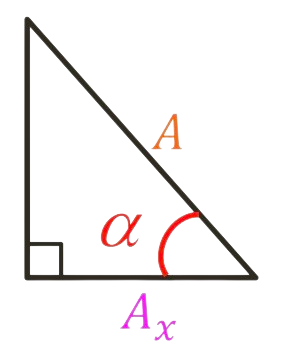
\includegraphics[width=2.5cm]{img/Ax.png}
    \end{center}
\end{theorem}

\section{Moment of forces}
\begin{definition}
    {Definition of moment}
    The moment of a force is a measure of its \emph{tendency} to cause a body to rotate about a specific point.

    The moment about a point $O$, when $F$ is applied a distance $d$ from the point is:
    \[M_O=F\times d\]
    Keep in mind that \emph{positive} moment is \emph{anti-clockwise}.
\end{definition}
\subsection{Coplanar / 2D moment}
\begin{knBox}
    {Resultant moments}
    The resultant moment is the \textbf{sum} of all moments present on the point, given by:
    \[M_R=\sum M_O\]
\end{knBox}
\subsubsection{The moment of a non-linearly attached force}
One simple way is to find the \emph{components} of the force, and sum their individual moments together. The following is a simple example:
\begin{center}
    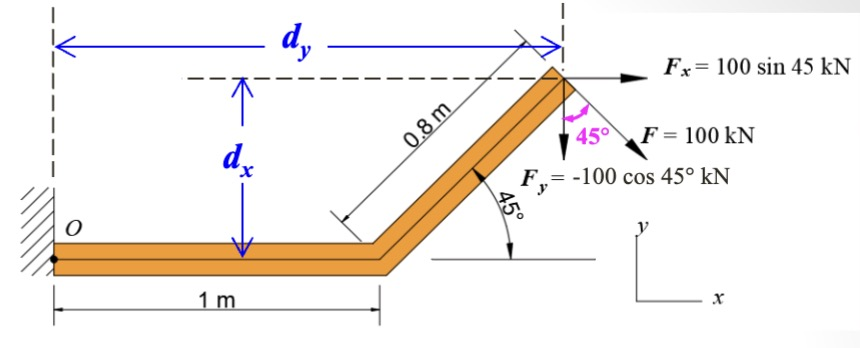
\includegraphics[width=8cm]{img/Moment1.jpg}

    After finding the component forces of $F$, we can deduce the resultant moment to be:
    \begin{align*}
        M_O & =F_x\times 0.8\sin 45\deg+F_y\times(1+0.8\cos 45\deg) \\
            & =-150.7kNm
    \end{align*}
\end{center}

\subsection{Non-coplanar / 3D moment}
\begin{definition}
    {Moments in a 3D system}
    Consider position vector $\vec{r}$ drawn from $O$ to \textbf{any point on the \emph{line of action}} of $F$. The moment can hence be given by:
    \[M_O=r\times F\]
\end{definition}
\begin{definition}
    {Finding the moment via cross products Cartesian vectors}
    The cross product $C$ given by $A$ and $B$ is:
    \[A\times B=\begin{vmatrix}
            i   & j   & k   \\
            A_x & A_y & A_z \\
            B_x & B_y & B_z
        \end{vmatrix}=C\]
    The cross-product for vectors going in the \emph{same direction} is 0. (i.e. $n\boldsymbol{k}\times m\boldsymbol{k}=0$)
\end{definition}
\begin{knBox}
    {Resultant moments}
    The resultant moment is simply the \textbf{sum} of \emph{couple moments} and moments of forces:
    \[(M_R)_O=\sum M_O + \sum M\]
    You can interpret $(M_R)_O$ as the resultant moment about point $O$.
\end{knBox}
\begin{knBox}
    {Finding moments by force perpendicular to plane}
    (Exam question) Given a force $F$ acting perpendicular to a plane $ABO$ at $O$, determine the moment about a point $A$.
    \begin{enumerate}
        \item Find the \emph{position vector} $\{r=OD\}$ of the force. ($AC\times BC=OD$)
        \item Convert force to Cartesian form. ($F=|F|\times\frac{r}{|r|}$)
        \item Find the \emph{cross product} of the vector from point to the force. ($M_A=OA\times F$)
    \end{enumerate}
\end{knBox}

\subsection{Couple moments}
Couples are \emph{two parallel forces} that have the same magnitude but have \emph{opposite directions}, separated by a \emph{perpendicular distance} $d$. The magnitude of the moment is given by:
\[M=Fd\]

\begin{minipage}{0.65\textwidth}
    Notice that there's no point mentioned so far. For couple moment, it is \textbf{always the same about any point}. Let's assume for any point $O$ (refer to graph), the moment is:
    \begin{align*}
        M_O & =r_B\times F+r_A\times -F \\&=(r_B-r_A)\times F\\&=r\times F\quad\text{which is independent of }O
    \end{align*}
    Hence, we can say that couple moments are \textbf{free vectors}.
\end{minipage}
\hfill
\begin{minipage}{0.3\textwidth}
    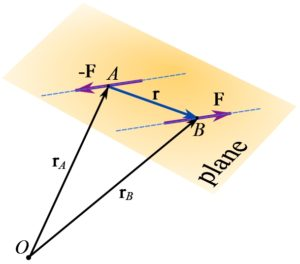
\includegraphics[width=0.95\textwidth]{img/Couple.jpg}
\end{minipage}



\section{Axially loaded members}
Axial loading refers to the application of a force along the axis of the member.
\subsection{Stress and strain}
\begin{definition}
    {Axial stress}
    Axial stress is the stress that is \emph{parallel} to the cross-sectional area of the member. It is given by:
    \[\sigma=\frac{F}{A}\quad(Nm^{-2})\]
    Where $F$ is the force applied, and $A$ is the cross-sectional area of the member. Note that $1 Pa = 1 Nm^{-2}$.
\end{definition}
\begin{theorem}
    {Eccentric loading and stress}
    When a force is applied \emph{off-centre} to the member, the stress at each end is given by:
    \[\sigma=\frac{\sum F}{wd}\pm \frac{6F\times e}{d\times w^2}\]
    Where $w$ is the width of the member, $d$ is the depth of the member, and $e$ is the eccentric distance from the centroid of the member to the point of application of the force.

    The $\pm$ sign is used to denote the \emph{maximum} and \emph{minimum} stress on opposite sides.
\end{theorem}
\begin{definition}
    {Axial strain}
    Axial strain is the ratio of the change in length to the original length of the member. It is given by:
    \[\epsilon=\frac{\Delta x}{x}\quad\text{(Ratio)}\]
    Where $\Delta x$ is the change in length, and $L$ is the original length of the member.
\end{definition}


\subsection{Materials}
\begin{definition}
    {Strength}
    Material strength is defined as the \textbf{maximum stress} that can be resisted by the material.
\end{definition}
\begin{definition}
    {Young's Modulus}
    Young's modulus is the ratio of stress to strain, given by:
    \[E=\frac{\sigma}{\epsilon}=\frac{Fx}{A\Delta x}\quad(Pa, Nm^{-2})\]
\end{definition}
\begin{definition}
    {Poisson's ratio}
    Poisson's ratio is the ratio of lateral strain $\epsilon_l$ to axial strain $\epsilon$, given by:
    \[\nu=-\frac{\epsilon_l}{\epsilon}\quad(\text{Ratio})\]
    \tcblower
    \begin{center}
        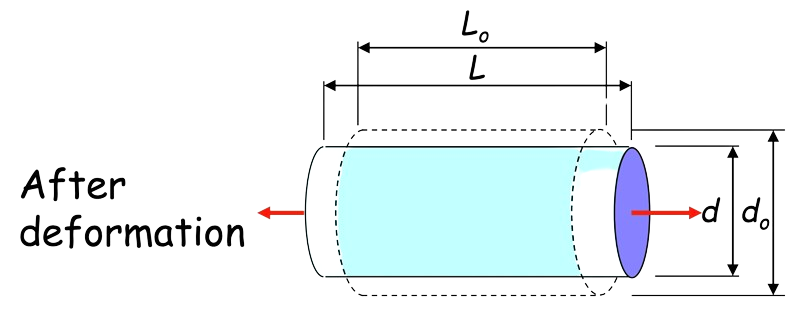
\includegraphics[width=0.5\textwidth]{./img/poisson.png}

        The lateral strain $\epsilon_l$ is $\frac{\Delta d}{d_0}$.
    \end{center}
\end{definition}

\subsection{Hydrostatic pressure}
\begin{definition}
    {Hydrostatic/water pressure}
    The water pressure acting on any surface is \emph{always perpendicular} to the surface, and the pressure is given by:
    \[p=\rho gh\quad(Pa, Nm^{-2})\]
    Where $\rho$ is the density of water,  and $h$ is the depth of the water.

    Hence, we can see that the water pressure \textbf{increases linearly with depth}.
\end{definition}
\begin{theorem}
    {Water pressure load on slanted surface}
    The load exerted on a slanted surface by water pressure F is given by and located at:
    \[F=\frac{\rho g d w L}{2}\quad @ \frac{1}{3}L\ /\ \frac{2}{3}d\]
    Where $d$ is the depth of water, $w$ is the width of the volume, and $L$ is the length of the surface.
\end{theorem}
\begin{definition}
    {Internal tensile stress}
    Internal tensile stress (hoop stress) refers to the stress caused by the internal force, acting along the \emph{circumferential direction} of a cross section. 
    \[\sigma_{\text{pipe}}=\frac{Pd}{2t},\quad\sigma_{\text{sphere}}=\frac{Pr}{2t}\]
    Where $P$ is the internal pressure, and $t$ is the thickness. 
    \begin{center}
        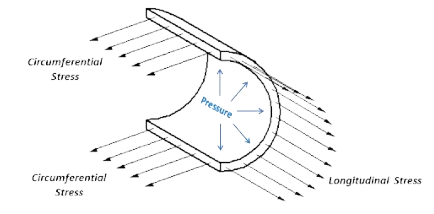
\includegraphics[width=0.7\textwidth]{./img/hoop.png}
    \end{center}
\end{definition}